\documentclass[a4paper,12pt]{article}

%%% Работа с русским языком
\usepackage{cmap}					% поиск в PDF
\usepackage{mathtext} 				% русские буквы в формулах
\usepackage[T2A]{fontenc}			% кодировка
\usepackage[utf8]{inputenc}			% кодировка исходного текста
\usepackage[english,russian]{babel}	% локализация и переносы
\usepackage{comment}


%%% Дополнительная работа с математикой
\usepackage{amsfonts,amssymb,amsthm,mathtools} % AMS
\usepackage{amsmath}
\usepackage{icomma} % "Умная" запятая: $0,2$ --- число, $0, 2$ --- перечисление

%% Номера формул
%\mathtoolsset{showonlyrefs=true} % Показывать номера только у тех формул, на которые есть \eqref{} в тексте.

%% Шрифты
\usepackage{euscript}	 % Шрифт Евклид
\usepackage{mathrsfs} % Красивый матшрифт

\usepackage{extsizes} % Возможность сделать 14-й шрифт
\usepackage{geometry} % Простой способ задавать поля
\geometry{top=25mm}
\geometry{bottom=35mm}
\geometry{left=20mm}
\geometry{right=20mm}

\usepackage{chngcntr}
\usepackage{hyperref}

\usepackage{setspace} % Интерлиньяж
%\onehalfspacing % Интерлиньяж 1.5
%\doublespacing % Интерлиньяж 2
%\singlespacing % Интерлиньяж 1

\usepackage{lastpage} % Узнать, сколько всего страниц в документе.
\usepackage{soulutf8} % Модификаторы начертания

\counterwithin*{equation}{section}
\counterwithin*{equation}{subsection}



%% Свои команды
\DeclareMathOperator{\sgn}{\mathop{sgn}}

%% Перенос знаков в формулах (по Львовскому)
\newcommand*{\hm}[1]{#1\nobreak\discretionary{}
	{\hbox{$\mathsurround=0pt #1$}}{}}

%%% Работа с картинками
\usepackage{graphicx}  % Для вставки рисунков
\graphicspath{{images/}{images2/}}  % папки с картинками
\setlength\fboxsep{3pt} % Отступ рамки \fbox{} от рисунка
\setlength\fboxrule{1pt} % Толщина линий рамки \fbox{}
\usepackage{wrapfig} % Обтекание рисунков и таблиц текстом

%%% Работа с таблицами
\usepackage{array,tabularx,tabulary,booktabs} % Дополнительная работа с таблицами
\usepackage{longtable}  % Длинные таблицы
\usepackage{multirow} % Слияние строк в таблице
\usepackage{graphicx}
\usepackage{fancyhdr}
\usepackage{hyperref}
\usepackage{booktabs}

\newcommand{\lt}{\left}
\newcommand{\rt}{\right}
\newcommand{\al}{\alpha}

\pagestyle{fancy}
\fancyhf{}
\pagestyle{plain} % нумерация вкл.

\rhead{\today}
\lhead{Соколов Игорь, группа 573}

%%% Заголовок
\author{Соколов Игорь, группа 573}
\title{ДЗ 4 по Методам Оптимизации. \newline Сопряженные множества. Двойственные конусы. Многогранники. Лемма Фаркаша}
\date{\today}

\begin{document} % конец преамбулы, начало документа	
	\maketitle
	
	\section{}
	
	Найти и изобразить на плоскости множество, сопряженное к многогранному конусу: $$ S = \mathbf{conv} \left\{ (-4,-1), (-2,-1), (-2,1)\right\} + \mathbf{cone} \left\{ (1,0), (2,1)\right\} $$
	
	\vspace{\baselineskip}
	
	\textbf{Решение:}
	
	Приведем теорему из семинара:
	
	Пусть $x_1,\ldots,x_m \in\mathbb{R}^n$. Сопряженным к многогранному множеству:
	$$ \textbf{S} = \mathbf{conv}\{x_1, \ldots, x_k\} + \mathbf{cone}\{x_{k+1}, \ldots, x_m \}$$
	
	является полиэдр (многогранник):
	\[\mathbf{S}^* = \left\{p \in \mathbb{R}^n \mid \langle{ p, x_i }\rangle \ge -1, i = \overline{1, k}; \langle{ p, x_i }\rangle \ge 0 , i =\overline{k+1, m} \right\} \]
	
	Используя теорему:
	\[\mathbf{S}^* = \{\mathbf{p} \in \mathbb{R}^n \mid -4p_1 - p_2 \ge -1\textbf{,} - 2p_1 -p_2 \ge -1\textbf{,} -2p_1 + p_2 \ge -1 \textbf{,} p_1 \ge 0 \textbf{,} 2p_1 + p_2 \ge 0\}\]
	
	Таким образом имеем систему:
	\[
	\left\{
	\begin{aligned}
	p_2 &\leq -4p_1 + 1  \\
	p_2 &\leq -2p_1 + 1\\
	p_2 &\ge 2p_1 - 1\\
	p_1 &\ge 0  \\
	p_2 &\ge -2p_1
	\end{aligned}
	\right.
	\]
	
	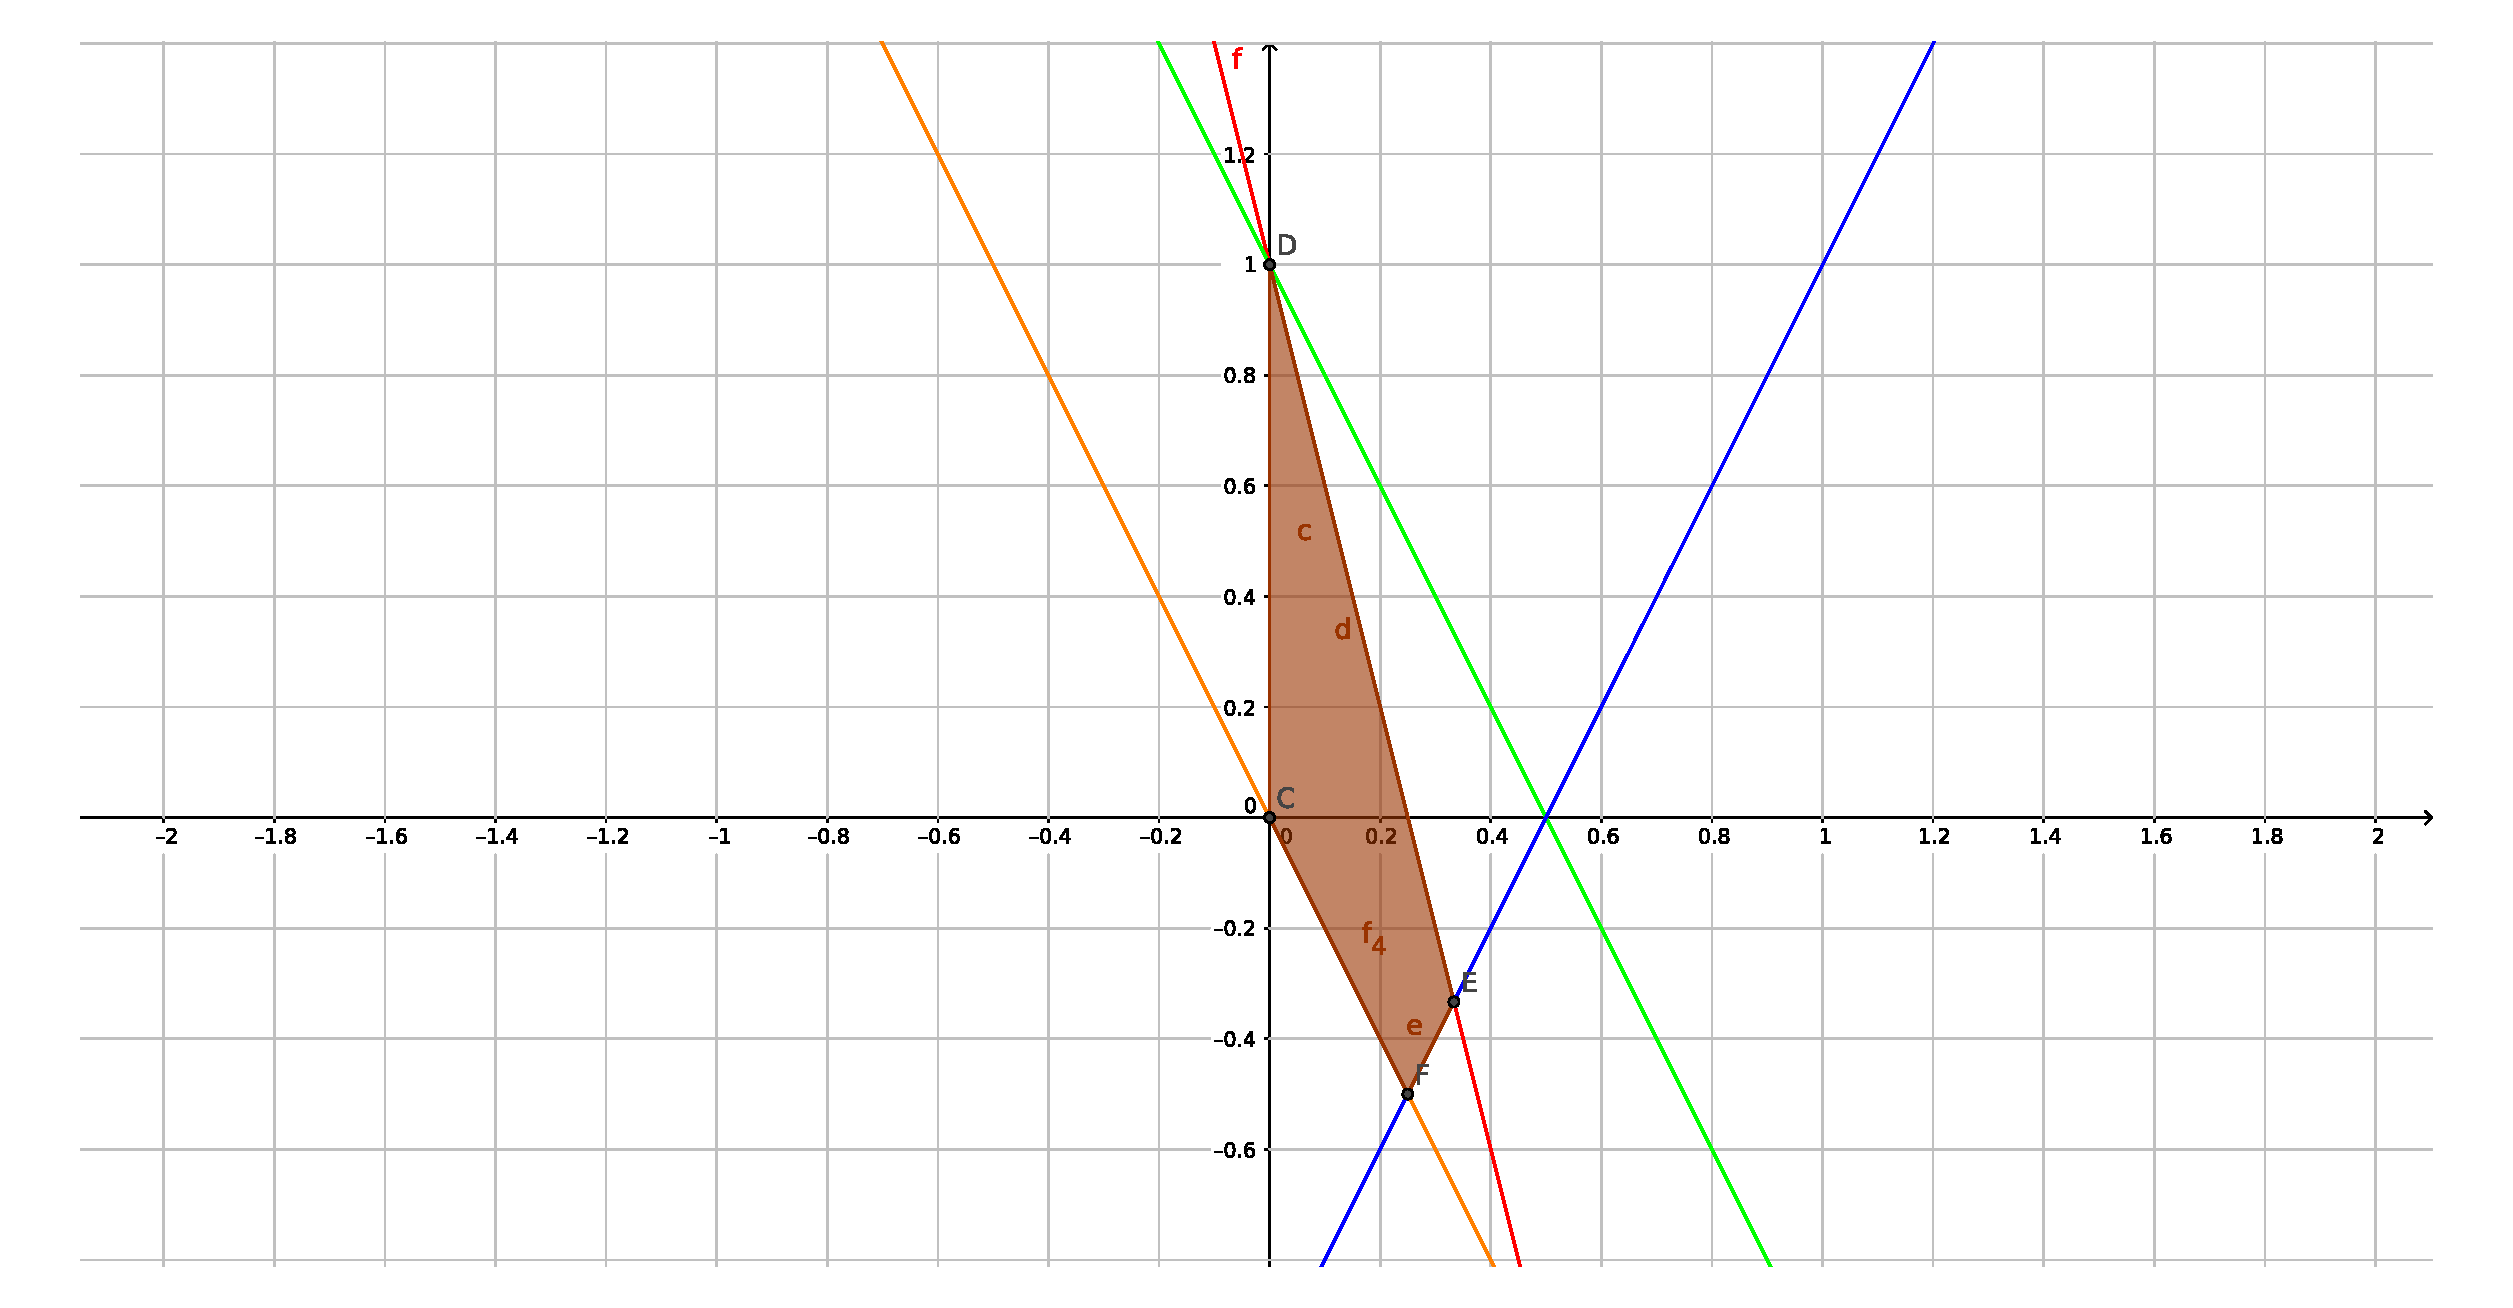
\includegraphics[width=\textwidth]{image_problem1.pdf}
	
	\vspace{\baselineskip}
	
	\section{}
	
	Найти и изобразить на плоскости множество, сопряженное к полиэдру: $$S = \left\{ x \in \mathbb{R}^2 \mid -3x_1 + 2x_2 \le 7, x_1 + 5x_2 \le 9, x_1 - x_2 \le 3, -x_2 \le 1\right\}$$
	
	\vspace{\baselineskip}
	
	\textbf{Решение:}
	
	\vspace{\baselineskip}
	
	Изобразим множество S на плоскости.
	
	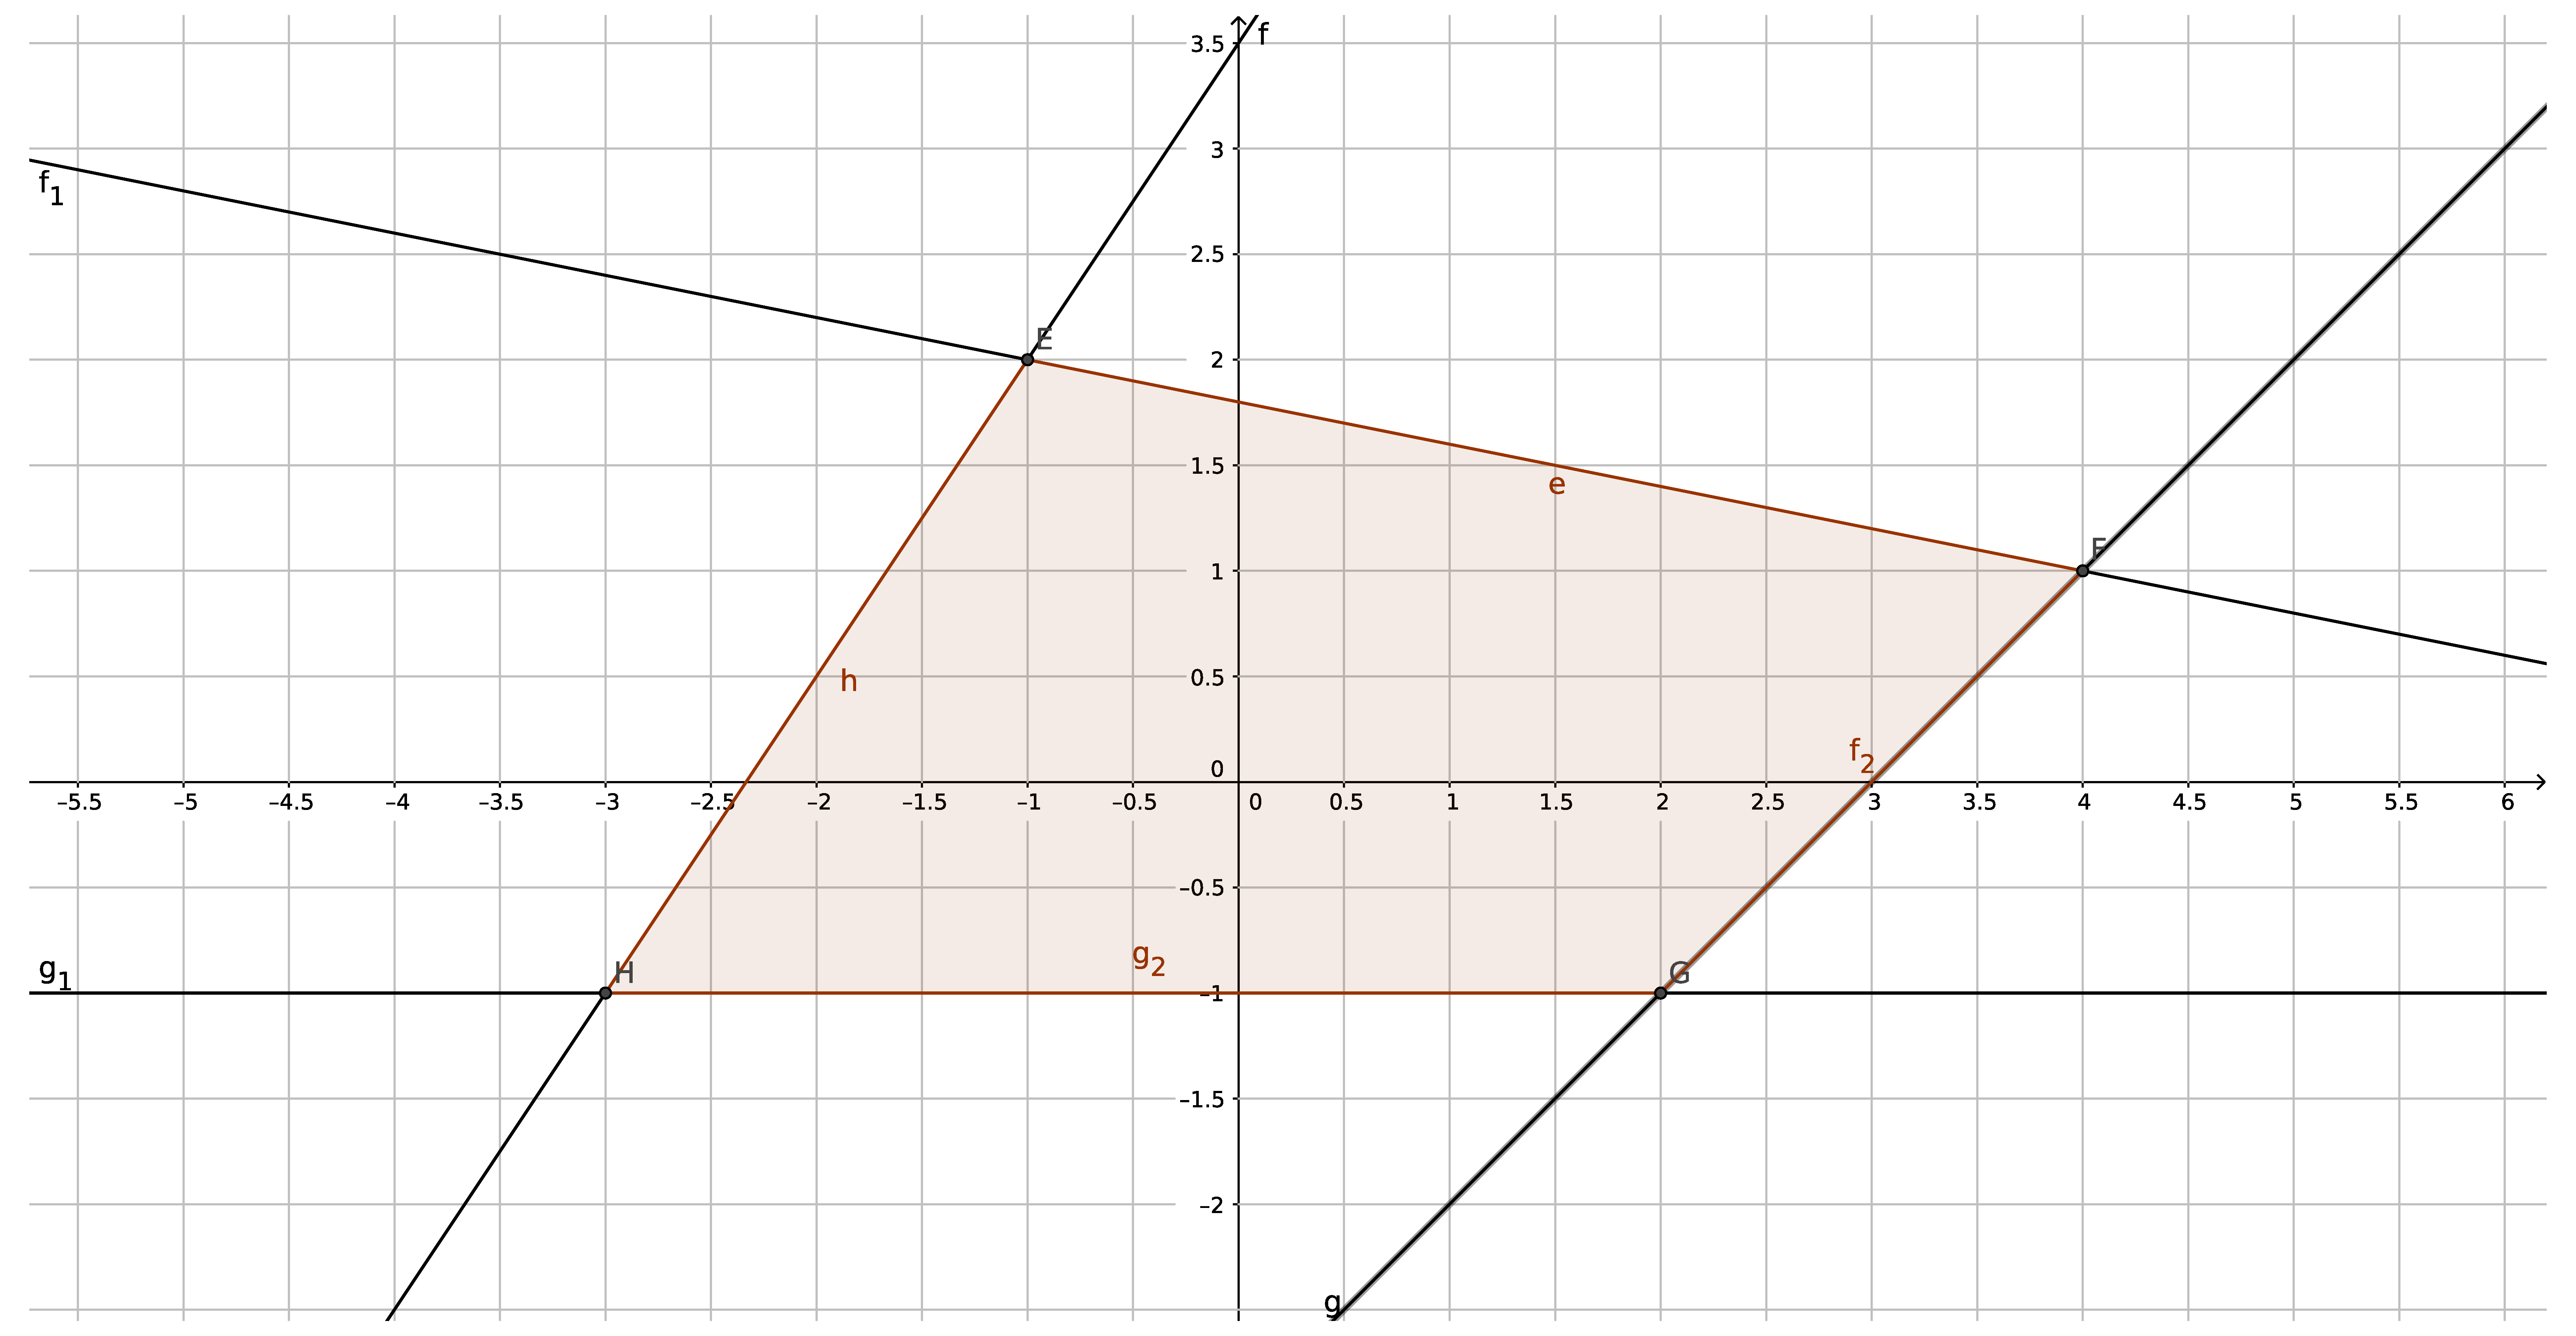
\includegraphics[width=\textwidth]{image_problem2.pdf}
	
	S задается системой: 
	
	\[
	\left\{
	\begin{aligned}
	-3x_1 + 2x_2 \le 7  \\
	 x_1 + 5x_2 \le 9\\
	x_1 - x_2 \le 3\\
	-x_2 \le 1 
	\end{aligned}
	\right.
	\]
	
	Пусть 
	
	$H = \begin{pmatrix}
	-3\\
	-1
	\end{pmatrix}$ точка пересечения прямых
	$
	\lt\{\begin{aligned}
		-3x_1 + 2x_2 = 7  \\
		-x_2 = 1 
	\end{aligned}
	\rt.
	$
	
	$E = \begin{pmatrix}
	-1\\
	2
	\end{pmatrix}$ точка пересечения прямых
	$
	\lt\{\begin{aligned}
	-3x_1 + 2x_2 = 7  \\
	x_1 + 5x_2 = 9
	\end{aligned}
	\rt.
	$
	
	$F = \begin{pmatrix}
	4\\
	1
	\end{pmatrix}$ точка пересечения прямых
	$
	\lt\{\begin{aligned}
	x_1 + 5x_2 = 9  \\
	x_1 - x_2 = 3 
	\end{aligned}
	\rt.
	$
	
	$G = \begin{pmatrix}
	2\\
	-1
	\end{pmatrix}$ точка пересечения прямых
	$
	\lt\{\begin{aligned}
	x_1 - x_2 = 3  \\
	-x_2 = 1 
	\end{aligned}
	\rt.
	$
	
	Очевидно, что $S = \mathbf{conv}(H, E, F, G)$.
	
	Тогда по ранее приведенной теореме имеем:
	
	$$ \mathbf{S^*} = \left\{ \mathbf{p} \in \mathbb{R}^2 \mid -3p_1 -p_2\geq-1, -p_1 +2p_2\geq-1, p_1 -p_2\geq-1, -p_2\geq-1,   \right\}$$
	
	\[\left\{
	\begin{aligned}
		p_2 &\leq -3p_1 + 1  \\
		p_2 &\geq \frac{p_1}{2} -\frac{1}{2}\\
		p_2 &\le p_1 + 1\\
		p_2 &\le 1  
	\end{aligned}
	\right.
	\]
	
	
	Изобразим теперь множество $\textbf{S}$ и $ \mathbf{S^*}$ на плоскости.
	
	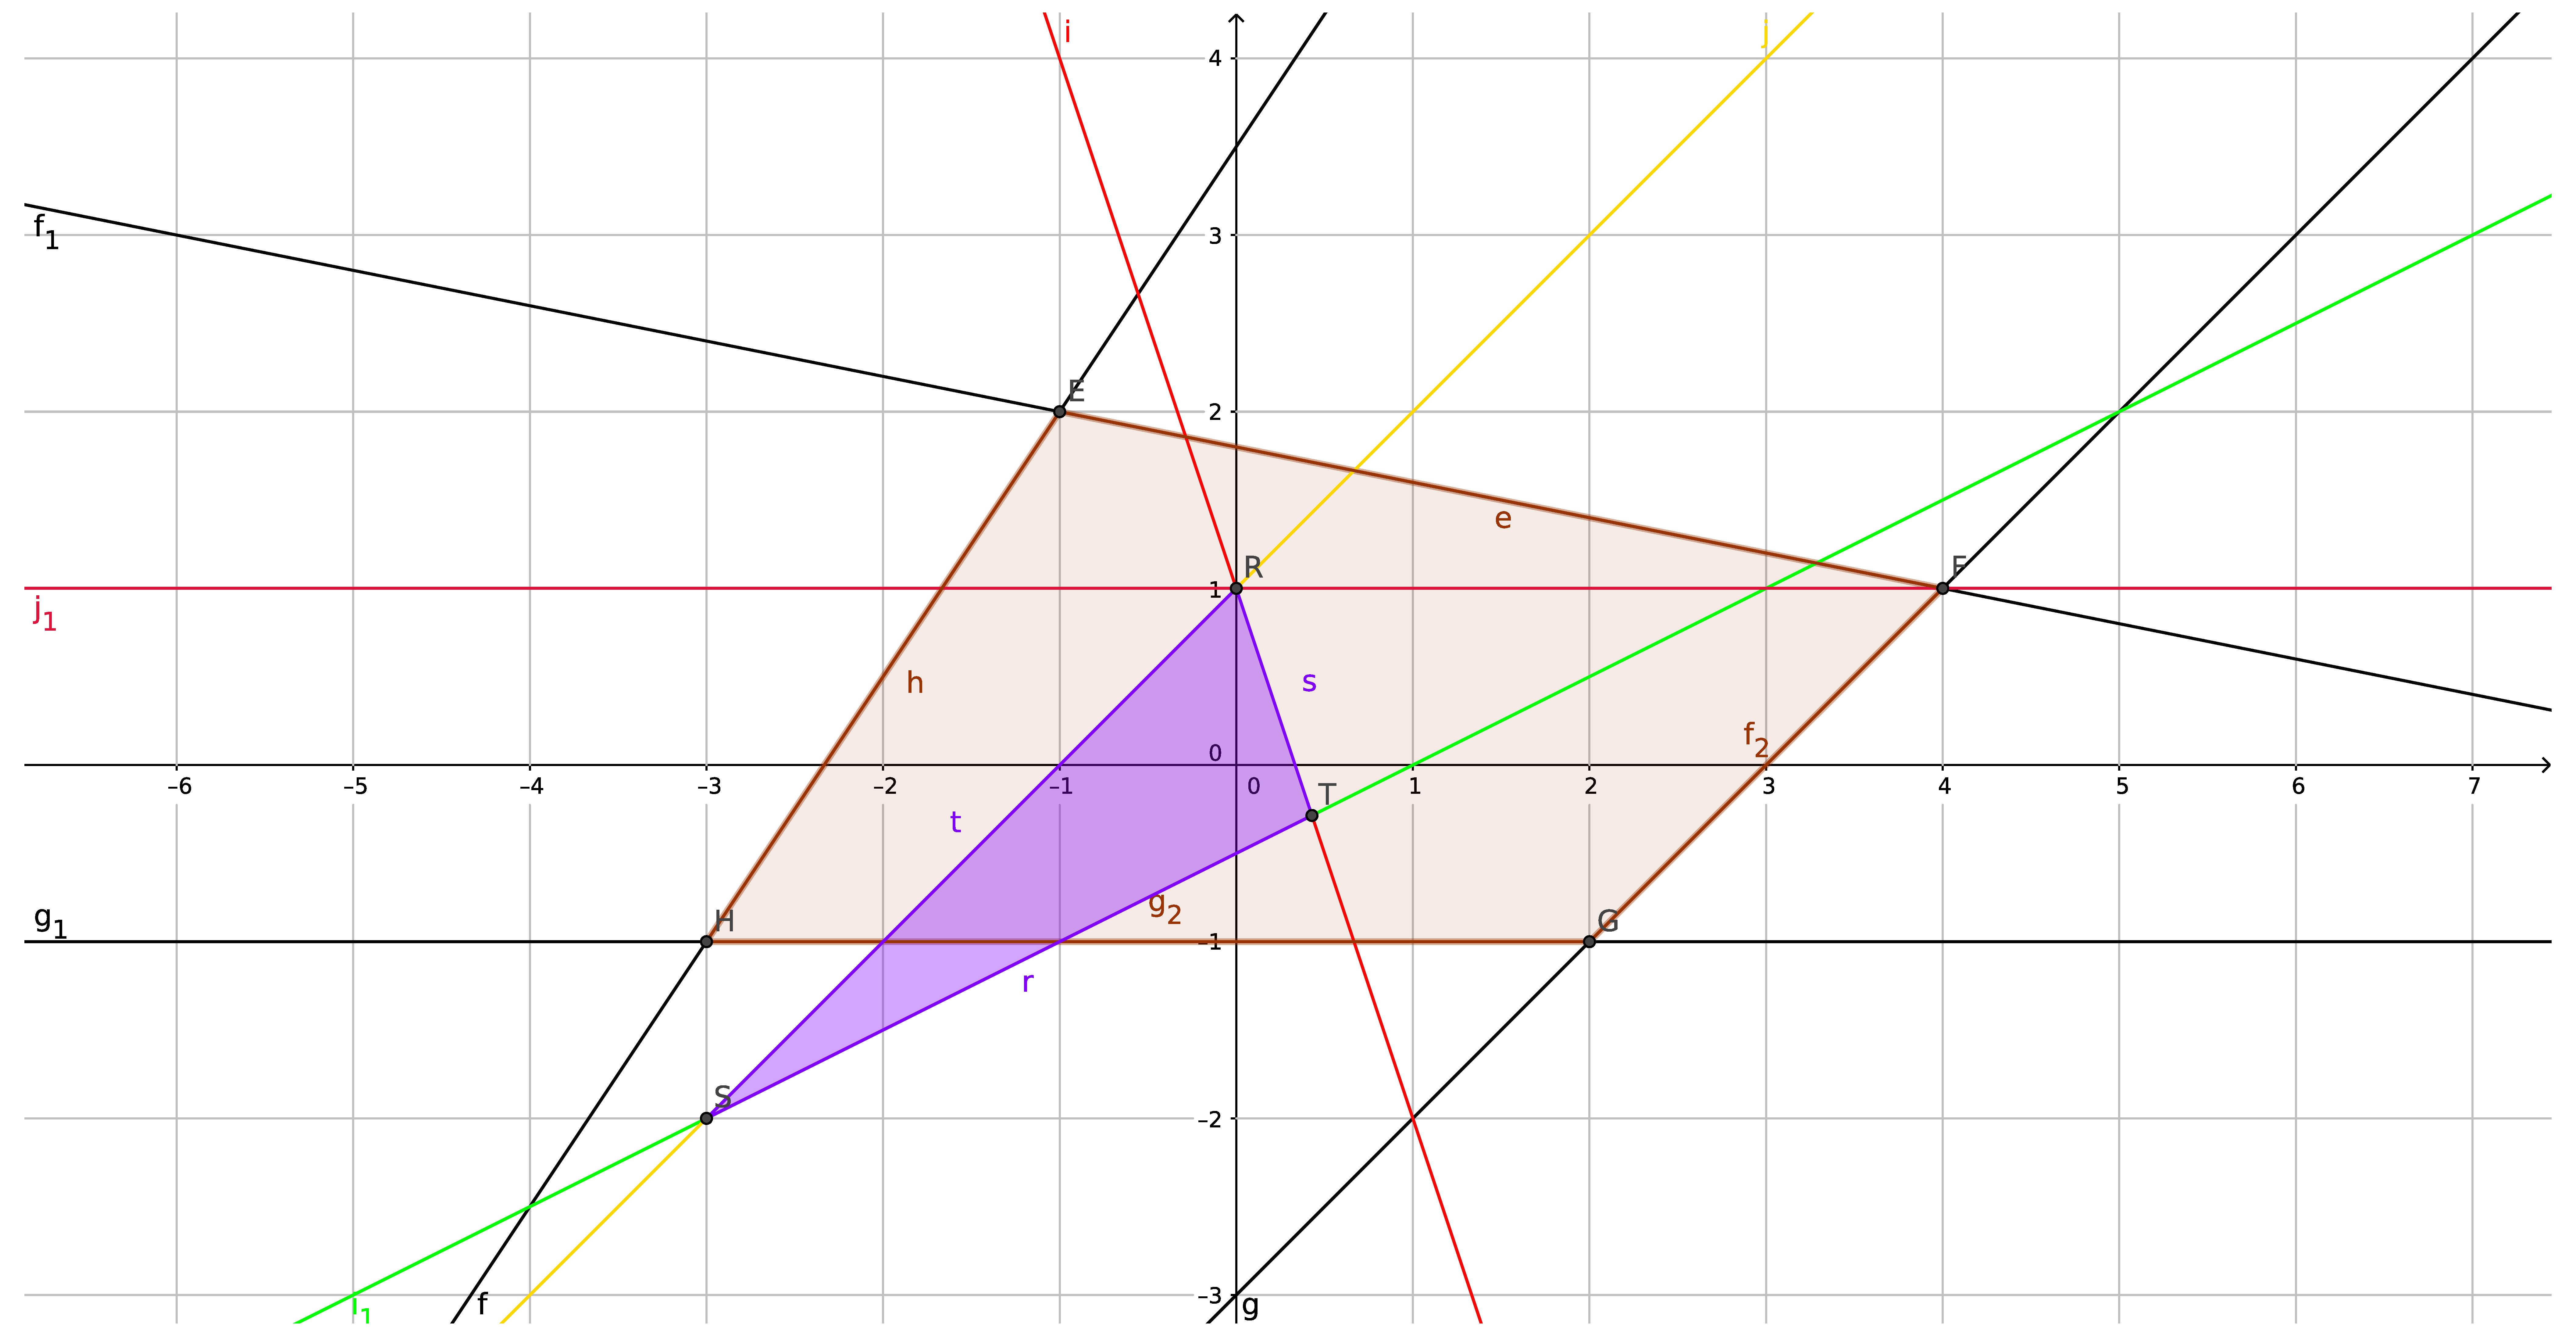
\includegraphics[width=\textwidth]{image2_problem2.pdf}
	
	%3
	
	\section{}
	
	Доказать, что если понятие сопряженного множества к множеству $S$ вводить как: $$S^* = \{y \ \in \mathbb{R}^n \mid \langle y, x\rangle \le 1 \;\; \forall x \in S\}, $$ то единичный шар с центром в нуле - единственное самосопряженное множество в $\mathbb{R}^n$.
	
	
	\begin{proof}
		
		Пусть $X = X^*$, $X^* = \{x \in \mathbb{R}^n \mid (x, x') \le 1,\ \forall x' \in X\}$. 
		
		Сначала докажем, что $X \subseteq B(0, 1)$. 
		
		Пусть $x \in X$, значит $x \in X^*$, значит $(x, x') \le 1,\ \forall x' \in X$, значит $(x, x) = \|x\| \le 1$, значит $x \in B(0, 1)$. 
		
		Теперь докажем, что $X \supseteq B(0, 1)$. Пусть $x \in B(0, 1)$. Пусть $x' \in X \subseteq B(0, 1)$, тогда по теореме Коши-Буняковского $(x, x') \le \|x\|\|x'\| \le 1$, значит $x \in X^* = X$
\end{proof}
	
	
	%4
	\section{}
	
	Найти множество, сопряженное к эллипсоиду: $$ S = \left\{ x \in \mathbb{R}^n \mid \sum\limits_{i = 1}^n a_i^2x_i^2 \le \varepsilon^2 \right\}$$
	
	\vspace{\baselineskip}
	
	\textbf{Решение:}
	
	\vspace{\baselineskip}
	
	\begin{equation}\label{s1}
	S = \left\{ x \in \mathbb{R}^n \mid \sum\limits_{i = 1}^n \frac{a_i^2}{\varepsilon^2}x_i^2 \le 1 \right\}
	\end{equation}
	
	1) Рассмотрим точки на $\partial S$.
		
	Для каждой точки $\mathbf{x} \in \partial S$ найдем уравнение касательной плоскости $\gamma$.
	
	\vspace{\baselineskip}
	
	$\nabla F (\mathbf{x}) = \lt(\dfrac{2a_1^2x_1}{\varepsilon^2}, \dots , \dfrac{2a_n^2x_n}{\varepsilon^2}\rt)^T$
	
	$\nabla F (\mathbf{x}) \lt( \mathbf{x} - \mathbf{y} \rt) = 0$, где $\mathbf{y} \in \gamma $
	
	Если записать 
	
	\begin{equation}\label{surface}	
	\nabla F (\mathbf{x}) \lt( \mathbf{x} - \mathbf{y} \rt) \le 0
	\end{equation}
	
	то данное неравенство описывает уже подпространство под плоскостью $\gamma$. 
	 
	Таким образом наше множество $S$ можно представить в виде множества пересекающихся подпространств, определяемых в каждой точке $\mathbf{x} \in \partial S $ касательной гиперплоскостью.
	
	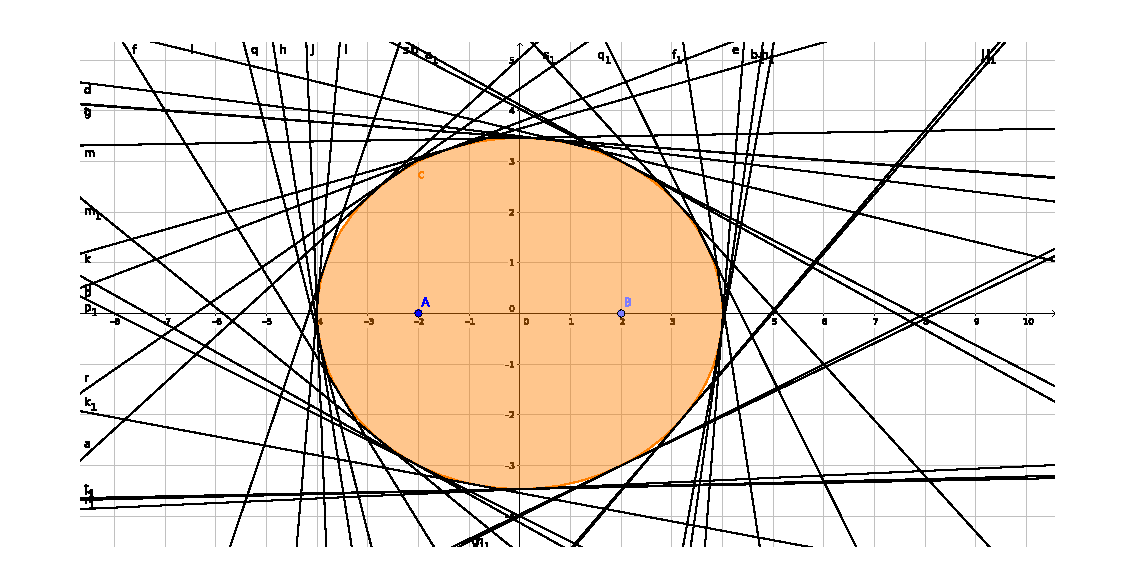
\includegraphics[width=\textwidth]{image_problem4.pdf}
	
	Из \eqref{surface}$\Rightarrow$ $S = \lt\{ \sum\limits_{i=1}^{n}\dfrac{2a_i^2}{\varepsilon^2} x_i (y_i - x_i) \le 0 \mid \forall \mathbf{x} \in \partial S , \rt\}$
	
	$$\sum\limits_{i=1}^{n}\dfrac{2a_i^2}{\varepsilon^2} x_iy_i \le \sum\limits_{i=1}^{n}\dfrac{2a_i^2}{\varepsilon^2}x_i^2$$
	
	Из \eqref{s1} $\Rightarrow \sum\limits_{i=1}^{n}\dfrac{a_i^2}{\varepsilon^2}x_i^2\le 1$
	
	
	$$\Rightarrow  \sum\limits_{i=1}^{n}\dfrac{2a_i^2}{\varepsilon^2} x_iy_i \le 2$$
	
	$$\sum\limits_{i=1}^{n}\dfrac{a_i^2}{\varepsilon^2} x_iy_i \le 1$$
	
	$$\sum\limits_{i=1}^{n}\lt[\lt(-\dfrac{a_i^2}{\varepsilon^2} y_i\rt)x_i\rt] \ge -1$$	
		
	\begin{equation}
	\Rightarrow \label{s3}
	\partial \mathbf{S}^* = \lt\{ \begin{pmatrix}
	-\dfrac{a_1^2}{\varepsilon^2} y_1\\
	\vdots\\
	-\dfrac{a_n^2}{\varepsilon^2} y_n
	\end{pmatrix}
	\Big| \sum\limits_{i=1}^{n}\lt[\lt(-\dfrac{a_i^2}{\varepsilon^2} y_i\rt)x_i\rt] \ge -1, \forall \mathbf{x} \in \partial \mathbf{S} \rt\}
	\end{equation}
	2) Покажем, что также верно 
	
	\begin{equation}\label{s4}
	\mathbf{S}^* = \lt\{ \begin{pmatrix}
	-\dfrac{a_1^2}{\varepsilon^2} y_1\\
	\vdots\\
	-\dfrac{a_n^2}{\varepsilon^2} y_n
	\end{pmatrix}
	\Big| \sum\limits_{i=1}^{n}\lt[\lt(-\dfrac{a_i^2}{\varepsilon^2} y_i\rt)x_i\rt] \ge -1, \forall \mathbf{x} \in  \mathbf{S} \rt\} 
	\end{equation}
	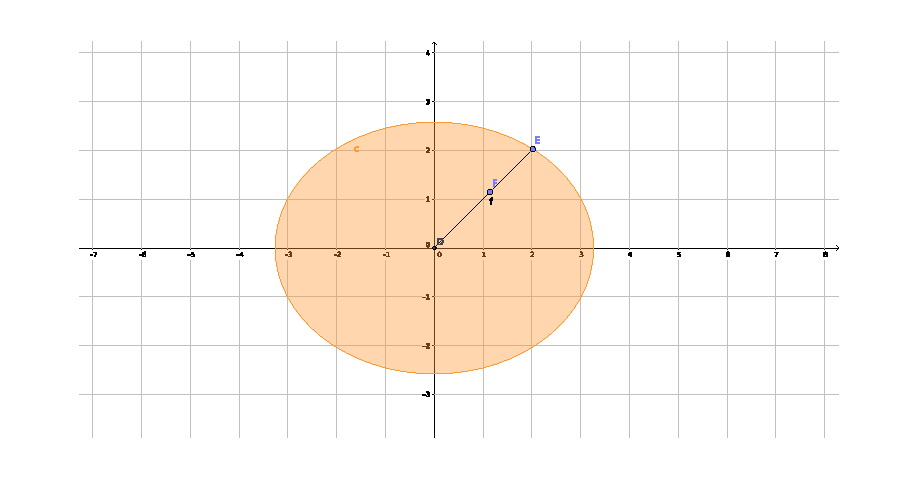
\includegraphics[width=\textwidth]{image3_problem4.pdf}
	\begin{equation}\label{s5}
	\sum\limits_{i=1}^{n}\lt[\lt(\dfrac{a_i^2}{\varepsilon^2} y_i\rt)x_i\rt] \le 1
	\end{equation}
	
	Возьмем $\mathbf{\widetilde{x}} = \theta \mathbf{x}, \forall \theta \in [0,1]$ (любая точка между на отрезке, соединяющий $\vec{0}$ и $\mathbf{x}$)
	
	$\Rightarrow \sum\limits_{i=1}^{n}\lt[\lt(\dfrac{a_i^2}{\varepsilon^2} y_i\rt)\widetilde{x_i}\rt] =\sum\limits_{i=1}^{n}\lt[\lt(\dfrac{a_i^2}{\varepsilon^2} y_i\rt)\theta x_i\rt]= \theta\sum\limits_{i=1}^{n}\lt[\lt(\dfrac{a_i^2}{\varepsilon^2} y_i\rt) x_i\rt] \le 1$
	
	$\Rightarrow \theta\sum\limits_{i=1}^{n}\lt[\lt(-\dfrac{a_i^2}{\varepsilon^2} y_i\rt) x_i\rt] \ge -1$
	
	$\Rightarrow \forall \mathbf{x} \in \partial S  \rightarrow \mathbf{\widetilde{x}} = \theta \mathbf{x} \in \mathbf{S^*}$
	
	 $\Rightarrow$ \eqref{s4} верно.
	 
	3) Покажем, что \eqref{s4} определяет некоторый эллипсоид.
	
	
	Из \eqref{s5} $\sum\limits_{i=1}^{n} y_i \lt(a_i^2 x_i\rt) \le \varepsilon^2$ - полупространство
	
	$\forall \mathbf{x} \in S \rightarrow \mathbf{x}\text{ и } \mathbf{y}$ лежат на одной касательной в точке $\mathbf{x}$ гиперплоскости.
	Рассмотрев по всем $\mathbf{x} \in \partial S$ снова получаем перечение полупространств, которые дают нам эллипсоид. 
	 
 
	
	
\end{document} % конец документа

